%-------------------------
% Resume in Latex
% Author 1chooo
% License : MIT
%------------------------

%---- Required Packages and Functions ----

\documentclass[a4paper,11pt]{article}
\usepackage{latexsym}
\usepackage{xcolor}
\usepackage{float}
\usepackage{ragged2e}
\usepackage[empty]{fullpage}
\usepackage{wrapfig}
\usepackage{lipsum}
\usepackage{tabularx}
\usepackage{titlesec}
\usepackage{geometry}
\usepackage{marvosym}
\usepackage{verbatim}
\usepackage{enumitem}
\usepackage[hidelinks]{hyperref}
\usepackage{fancyhdr}
\usepackage{fontawesome5}
\usepackage{multicol}
\usepackage{graphicx}
\usepackage{cfr-lm}
\usepackage[T1]{fontenc}
\setlength{\multicolsep}{0pt} 
\pagestyle{fancy}
\fancyhf{} % clear all header and footer fields
\fancyfoot{}
\renewcommand{\headrulewidth}{0pt}
\renewcommand{\footrulewidth}{0pt}
\geometry{left=1.4cm, top=0.8cm, right=1.2cm, bottom=1cm}
% Adjust margins
%\addtolength{\oddsidemargin}{-0.5in}
%\addtolength{\evensidemargin}{-0.5in}
%\addtolength{\textwidth}{1in}
\usepackage[most]{tcolorbox}
\tcbset{
	frame code={}
	center title,
	left=0pt,
	right=0pt,
	top=0pt,
	bottom=0pt,
	colback=gray!20,
	colframe=white,
	width=\dimexpr\textwidth\relax,
	enlarge left by=-2mm,
	boxsep=4pt,
	arc=0pt,outer arc=0pt,
}

\usepackage{enumitem}
\setlist[itemize]{label=-, leftmargin=0cm, itemsep=0cm, topsep=0cm}


\urlstyle{same}

\raggedright
\setlength{\tabcolsep}{0in}

% Sections formatting
\titleformat{\section}{
  \vspace{-4pt}\scshape\raggedright\large
}{}{0em}{}[\color{black}\titlerule \vspace{-7pt}]

%-------------------------
% Custom commands
\newcommand{\resumeItem}[2]{
  \item{
    \textbf{#1}{\hspace{0.5mm}#2 \vspace{-0.5mm}}
  }
}

\newcommand{\resumePOR}[3]{
\vspace{0.5mm}\item
    \begin{tabular*}{0.97\textwidth}[t]{l@{\extracolsep{\fill}}r}
        \textbf{#1}\hspace{0.3mm}#2 & \textit{\small{#3}} 
    \end{tabular*}
    \vspace{-2mm}
}

\newcommand{\resumeSubheading}[4]{
\vspace{0.5mm}\item
    \begin{tabular*}{0.98\textwidth}[t]{l@{\extracolsep{\fill}}r}
        \textbf{#1} & \textit{\footnotesize{#4}} \\
        \textit{\footnotesize{#3}} &  \footnotesize{#2}\\
    \end{tabular*}
    \vspace{-2.4mm}
}

\newcommand{\resumeProject}[4]{
\vspace{0.5mm}\item
    \begin{tabular*}{0.98\textwidth}[t]{l@{\extracolsep{\fill}}r}
        \textbf{#1} & \textit{\footnotesize{#3}} \\
        \footnotesize{\textit{#2}} & \footnotesize{#4}
    \end{tabular*}
    \vspace{-2.4mm}
}

\newcommand{\resumeSubItem}[2]{\resumeItem{#1}{#2}\vspace{-4pt}}

% \renewcommand{\labelitemii}{$\circ$}
\renewcommand{\labelitemi}{$\vcenter{\hbox{\tiny$\bullet$}}$}

\newcommand{\resumeSubHeadingListStart}{\begin{itemize}[leftmargin=*,labelsep=0mm]}
\newcommand{\resumeHeadingSkillStart}{\begin{itemize}[leftmargin=*,itemsep=1.7mm, rightmargin=2ex]}
\newcommand{\resumeItemListStart}{\begin{justify}\begin{itemize}[leftmargin=3ex, rightmargin=2ex, noitemsep,labelsep=1.2mm,itemsep=0mm]\small}

\newcommand{\resumeSubHeadingListEnd}{\end{itemize}\vspace{2mm}}
\newcommand{\resumeHeadingSkillEnd}{\end{itemize}\vspace{-2mm}}
\newcommand{\resumeItemListEnd}{\end{itemize}\end{justify}\vspace{-2mm}}
\newcommand{\cvsection}[1]{%
\vspace{2mm}
\begin{tcolorbox}
    \textbf{\large #1}
\end{tcolorbox}
    \vspace{-4mm}
}

\newcolumntype{L}{>{\raggedright\arraybackslash}X}%
\newcolumntype{R}{>{\raggedleft\arraybackslash}X}%
\newcolumntype{C}{>{\centering\arraybackslash}X}%
%---- End of Packages and Functions ------

%-------------------------------------------
%%%%%%  CV STARTS HERE  %%%%%%%%%%%
%%%%%% DEFINE ELEMENTS HERE %%%%%%%
\newcommand{\name}{Hugo ChunHo Lin} % Your Name
\newcommand{\course}{Dept. of Atmospheric Science, NCU.} % Your Program
\newcommand{\roll}{xxxxxxx} % Your Roll No.
\newcommand{\phone}{909-001068} % Your Phone Number
\newcommand{\emaila}{hugo970217@gmail.com} %Email 1
\newcommand{\emailb}{lcho0127@g.ncu.edu.tw} %Email 2
\newcommand{\myScore}{}
% \newcommand{\myScore}{GPA: 3.01/4.30; Rank: 25/33}


\begin{document}
\fontfamily{cmr}\selectfont
%----------HEADING-----------------


% \parbox{2.35cm}{%
% % 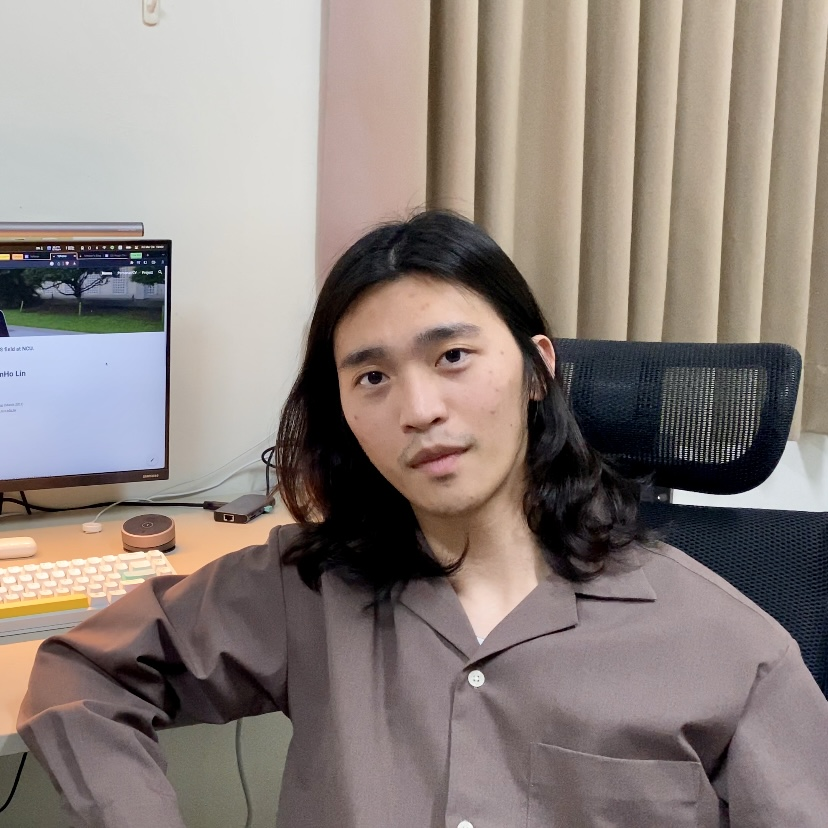
\includegraphics[width=2cm,clip]{IMG_4754.jpg}
% }
\parbox{\textwidth}{
\begin{tabularx}{\linewidth}{L r} \\
  \textbf{\huge \name} & {\raisebox{0.0\height}{\footnotesize \faPhone}\ +886-\phone}\\ Targeting \textbf{Amazon Web Services} from 2023.07.31-2024.01.31
   & \href{mailto:\emaila}{\raisebox{0.0\height}{\footnotesize \faEnvelope}\ {\emaila}} \\
  XinYi, Taipei, Taiwan. & \href{https://sites.google.com/g.ncu.edu.tw/1chooo/portfolio}{\raisebox{0.0\height}{\footnotesize \faGlobe}\ {1chooo's Portfolio}}\\
  {Major: \course} &  \href{https://github.com/1chooo}{\raisebox{0.0\height}{\footnotesize \faGithub}\ {1chooo}} \\
  {Minor Specialty: Dept. of CSIE, NCU.} & \href{https://www.linkedin.com/in/1chooo/}{\raisebox{0.0\height}{\footnotesize \faLinkedin}\ {Hugo ChunHo Lin}}
\end{tabularx}
}
% \parbox{3.0cm}{%
% \flushright 
\includegraphics[width=2cm,clip]{nitp_logo.png}
% }

%-----------EDUCATION-----------------
\section{\textbf{Education}}
  \resumeSubHeadingListStart
    \resumeSubheading
      { National Central University}{\myScore}
      {Junior Student who possesses a true passion for the CS field.}{Sep. 2020 - present}
      \vspace{-1.0mm}
      \resumeItemListStart
        \item {Major: Department of Atmospheric Science}
        \item {Minor: Department of Computer Science \& Information Engineering}
        \item {Course: Alg, DS, Assembly, PPL, Degital Design, Weather and AI, etc.}
      \resumeItemListEnd      
  \resumeSubHeadingListEnd
\vspace{-5.5mm}


%-----------EXPERIENCE-----------------
\section{\textbf{Work Experience}}
  \resumeSubHeadingListStart
    \resumeSubheading
    { Pegatron Corporation}{}
    {}{}
    \vspace{-4.0mm}
    \resumeItemListStart
    
    \begin{itemize}[leftmargin=0cm, itemsep=0cm, topsep=0cm]

    \item \parbox{\dimexpr\linewidth-4cm\relax}{\textbf{Software Engineer Summer Intern} \textbf{}}
          \textit{\footnotesize{\hfill Jul. 2023 - present}}
    
     \hspace{0.5cm}\parbox{\dimexpr\linewidth -1cm\relax}{\footnotesize{Practical Project: Implementing Defect Detection using Machine Learning in the Scrum Method.}}

    \end{itemize}

    \resumeItemListEnd
    
    \vspace{-3.0mm}
    \resumeSubheading
    { Teaching Assistant, NCU}{}
    {}{}
    \vspace{-4.0mm}
    \resumeItemListStart
    
    \begin{itemize}[leftmargin=0cm, itemsep=0cm, topsep=0cm]

    \item \parbox{\dimexpr\linewidth-4cm\relax}{\textbf{Course:} \textbf{}Freshman English.}
          \textit{\footnotesize{\hfill Aug. 2022 - Jun. 2023}}
    
    \hspace{0.5cm}\parbox{\dimexpr\linewidth -1cm\relax}{\footnotesize{Design a lesson that will allow us to interact with students entirely in English.}}
     
     \hspace{0.5cm}\parbox{\dimexpr\linewidth -1cm\relax}{\footnotesize{Stay up-to-date with the latest global developments and trends.}}
    \item \parbox{\dimexpr\linewidth-4cm\relax}{\textbf{Course:} \textbf{}Student Service-Learning.}
          \textit{\footnotesize{\hfill Feb. 2021 - Jun. 2021}}

    \hspace{0.5cm}\parbox{\dimexpr\linewidth -1cm\relax}{\footnotesize{Led beach cleaning initiative to promote environmental awareness and conservation efforts}}
     
     \hspace{0.5cm}\parbox{\dimexpr\linewidth -1cm\relax}{\footnotesize{Created Earth Science education program for elementary schools.}}
    

    \end{itemize}

    \resumeItemListEnd
    
    \vspace{-3.0mm}

    \resumeSubheading
    { Center for Teaching Education, NCU}{}
    {}{}
    \vspace{-4.0mm}
    \resumeItemListStart
        % {\textbf{Website Administrator.}}{}
    \begin{itemize}[leftmargin=0cm, itemsep=0cm, topsep=0cm]
    \item \parbox{\dimexpr\linewidth-4cm\relax}{\textbf{Website Administrator} }
          \textit{\footnotesize{\hfill July. 2022 - Jan. 2023}}

    \hspace{0.5cm}\parbox{\dimexpr\linewidth -1cm\relax}{\footnotesize{Manage website data and maintain the server.}}
     
     \hspace{0.5cm}\parbox{\dimexpr\linewidth -1cm\relax}{\footnotesize{Launch a project aimed at developing a system to manage and track student progress.}}
    % \item \parbox{\dimexpr\linewidth-4cm\relax}{Manage website data and maintain the server.}
    % \item \parbox{\dimexpr\linewidth-4cm\relax}{Launch a project aimed at developing a system to manage and track student progress.}

    \end{itemize}

    \resumeItemListEnd

      
  \resumeSubHeadingListEnd
\vspace{-5.5mm}

\section{\textbf{Extracurricular Activity}}
  \resumeSubHeadingListStart
    \resumeSubheading
      {{\href{https://ncufresh22tmp.le37.tw/blog/}{ NCUFresh Team(NCUBlog)}}}{}
      {Website developer team for the incoming freshmen admitting to NCU.}{Dec. 2021 - Jul. 2022}
      \vspace{-1.0mm}
      \resumeItemListStart
        \item {The essential experience of manage larger projects with teammates.}
        \item {Frontend skills: UI/UX, Figma.}
        \item {Teamwork: leadership, meeting arrangement, facilitating communication, project demo.}
        \item {Marketing: increase social media reach, content of films and articles.}
      \resumeItemListEnd
    
    \vspace{-3.0mm}
    
    
    \resumeSubheading
      {{\href{https://github.com/NCUAppTeam}{ NCUApp Team(UI/UX \& Marketing)}}}{}
      {The app developer team opens to all members of the NCU community.}{Mar. 2023 - present}
      \vspace{-1.0mm}
      \resumeItemListStart
        \item {The crucial experience managing existing projects with teammates to ensure that all functions are fully developed.}
        \item {Frontend skills: React Native, UI/UX, Figma.}
        \item {Marketing: product listings, map functionality, daily scheduling.}
      \resumeItemListEnd
    \vspace{-3.0mm}
    
    
    \resumeSubheading
      { Co-captain(Basketball Team)}{}
      {Basketball Team Co-captain in my department, Dept. ATM, NCU.}{Aug. 2022 - present}
      \vspace{-2.0mm}
      \resumeItemListStart
    % \item {Work description line 1}
    % \item {Work description line 2}
    \resumeItemListEnd
      
  \resumeSubHeadingListEnd

      
      
  % \resumeSubHeadingListEnd
\vspace{-5.5mm}



%-----------PROJECTS-----------------
\section{\textbf{Projects Relating to AWS}}
\resumeSubHeadingListStart

    \resumeProject
      {\href{https://www.youtube.com/watch?v=S0HZJIqVThI}{ BearBear You}} %Project Name
      {Develop a Line BOT utilizing \textbf{S3 and Amazon Recognition services} to enhance familiarity with NCU Campus.} %Project Name, Location Name
      {Jun. 2022} %Event Dates

        \vspace{-2mm}

      \resumeItemListStart
        \item {Training Model with Amazon Recognition and storing training data to AWS S3.}
        \item {Integrating with Line BOT using \textbf{Python Line Bot SDK and Flask}.}
        \item {Create an engaging storyline or narrative that enhances user interaction and exploration of the Central Campus.}
        \item {Demo Video: {\href{https://www.youtube.com/watch?v=S0HZJIqVThI}{LINE BOT \textbf{BearBear You} - Demo}} }
        \item {Story Flow: {\href{https://1chooo.notion.site/GS3073B-IntroToAI-a1a08a8c940f4d46ad89fc28b30fa33a?pvs=4}{LINE BOT \textbf{BearBear You} - Story Flow}} }
    \resumeItemListEnd
    \vspace{-3mm}
    
  \resumeSubHeadingListEnd
  \vspace{-5.5mm}
  
  
  %-----------Technical skills-----------------
  % \section{\textbf{Technical Skills and Interests}}
  \section{\textbf{Skills}}
  \begin{itemize}[leftmargin=0.05in, label={}]
    \vspace{1.0mm}
    {\item{
      \textbf{Programming Languages}{: Python, c/c++, Java, Assembly, JavaScripts, LaTeX, etc.} \\
      \textbf{ML/DL}{: Keras, Tensorflow, Scikit-learn, Numpy, Pandas, etc.} \\
      \textbf{Cloud/Databases}{: AWS(S3, Amazon Rekognition), mySQL.} \\
      \textbf{Soft Skills}{: Git, GUI, line bot, blog.} \\
      \textbf{Languages}{: English(TOEIC 690 - Listening: 355; Reading: 335, Mar. 2023), Mandarin.} \\
    }}

 \end{itemize}
 % \vspace{-16pt}

%-------------------------------------------
\end{document}


